\subsection{Laurent Expansions}
Suppose $f$ is any function on an open subset of the complex plane. Then we say $f$ has a Laurent expansion if there exist $a_n$ for $n \in \Z$ so that
$$ f(z) = \sum_{n = - \infty}^\infty a_n z^n $$
One might wonder how to interpret this sum and what it means for such a sum to be convergent. One natural way to think about this sum is to consider the positive and negative indices separately. In other words, we will say that 
$$ \sum_{n = - \infty}^\infty a_n z^n = \sum_{n \geq 0} a_n z^n + \sum_{n < 0} a_n z^n $$
\begin{remark}
Note the similarity to $\displaystyle \int_{-\infty}^{\infty}$.
\end{remark}
The convergence of the second term above can be understood by considering whether it converges in $\zeta$ for $z = \frac{1}{\zeta}$ (this gets us back to a series with positive powers).

\begin{proposition}
Suppose $f$ is a holomorphic function on an annulus $A := \{0 \leq R_2 < \abs{z} < R_1 \leq \infty\}$. Then $f$ has a convergent Laurent expansion in the annulus.
\end{proposition}
\begin{proof}
Suppose $z$ is any point in $A$.
Choose $r_1, r_2$ such that $R_2 < r_2 < \abs{z} < r_1 < R_1$. Let $K$ denote the closed annulus corresponding to this choice of $r_1, r_2$. In other words, $K := \{z \in \C : r_2 \leq \abs{z} \leq r_1\}$. Let $D$ be a small closed disk centered at $z$ that is contained in $K$. Then $\frac{f(\zeta)}{\zeta - z}$ is holomorphic on $K \setminus D$. Therefore by Cauchy's Theorem we get
$$ \int_{\partial(K \setminus D)} \frac{f(\zeta)}{\zeta - z} d\zeta = 0$$
($\frac{f(\zeta)}{\zeta - z} d\zeta$ is closed so by Stokes' Theorem we get that the above integral is 0). In particular, then we conclude that
$$ \int_{\partial K} \frac{f(\zeta)}{\zeta - z} d\zeta = \int_{\partial D} \frac{f(\zeta)}{\zeta - z} d\zeta = f(z) 2\pi i $$
where the final equality follows from Cauchy's Integral Formula. Thus overall we conclude that
$$f(z) = \frac{1}{2\pi i} \int_{\partial K} \frac{f(\zeta)}{\zeta - z}d\zeta = \frac{1}{2\pi i} \int_{\abs{\zeta} = r_1} \frac{f(\zeta)}{\zeta - z} d\zeta - \frac{1}{2\pi i} \int_{\abs{\zeta} = r_2} \frac{f(\zeta)}{\zeta - z} d\zeta$$
Let $\gamma_1$ denote the circle of radius $r_1$ and $\gamma_2$ the circle of radius $r_2$.

\begin{figure}
    \centering    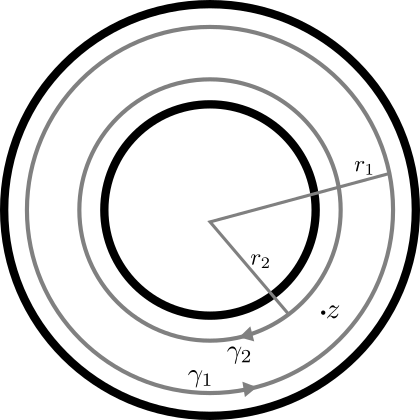
\includegraphics{Images/laurent_expansion_annulus.png}
    \caption{Laurent expansion in an annulus}
    \label{fig:laurent-expansion-annulus}
\end{figure}

We know the first integral can be written as an infinite sum since 
\begin{align*}
    \int_{\gamma_1} \frac{f(\zeta)}{\zeta - z} d\zeta &= \int_{\gamma_1} \frac{f(\zeta)}{\zeta} \cdot \frac{1}{1 - \frac{z}{\zeta}} d\zeta\\
    &= \int_{\gamma_1} \frac{f(\zeta)}{\zeta} \sum_{n = 0}^\infty \left( \frac{z}{\zeta} \right)^n d\zeta\\
    &= \sum_{n = 0}^\infty \left( \int_{\gamma_1} \frac{f(\zeta)}{\zeta^{n + 1}} \right) z^n
\end{align*}
For the second integral, we do something similar
\begin{align*}
    -\int_{\gamma_2} \frac{f(\zeta)}{\zeta - z} d\zeta &= \int_{\gamma_2} -\frac{f(\zeta)}{z} \cdot \frac{1}{1 - \frac{\zeta}{z}} d\zeta\\
    &= \int_{\gamma_2} \frac{f(\zeta)}{z} \sum_{n = 0}^\infty \left(\frac{\zeta}{z}\right)^n d\zeta\\
    &= \int_{\gamma_2} f(\zeta) \sum_{n = 0}^\infty \frac{\zeta^n}{z^{n + 1}} d\zeta \\
    &= \int_{\gamma_2} f(\zeta) \sum_{n = 1}^\infty \frac{\zeta^{n - 1}}{z^n} d\zeta \\
    &= \int_{\gamma_2} f(\zeta) \sum_{n < 0} \frac{\zeta^{-n - 1}}{z^{-n}} d\zeta\\
    &= \int_{\gamma_2} f(\zeta) \sum_{n < 0} \frac{z^n}{\zeta^{n + 1}} d\zeta \\
    &= \sum_{n < 0} \left( \int_{\gamma_2} \frac{f(\zeta)}{\zeta^{n + 1}} \right) z^n 
\end{align*}

We see that the coefficients are (almost) the exact same. The only difference is the curve we integrate over. Thus we can write the Laurent expansion quite succinctly as 
$$ f(z) \sum_{n = -\infty}^{\infty} a_n z^n $$
where
$$ a_n = \frac{1}{2\pi i} \int_{\gamma_i} \frac{f(\zeta)}{\zeta^{n + 1}} d\zeta $$
so that $i = 1$ if $n \geq 0$ and $i = 2$ if $n < 0$.
This series converges uniformly and absolutely for $r_2 \leq \abs{z} \leq r_1$ where $R_2 < r_2 < r_1 < R_1$. 
\end{proof}

Above we looked at a general annulus but a particularly interesting and important case is that of the punctured neighbourhood, i.e. when $R_2 = 0$. For example, we might have a holomorphic function $f(z)$ in a punctured disk centered at 0. Then we say that $f(z)$ has an isolated singularity at $z = 0$ if it can't be extended to a holomorphic function on the entire disk. The statement below tells us exactly when this is possible.
\begin{proposition}\label{prop:holom-extend}
Suppose $f$ is a holomorphic function on the punctured disk $0 < \abs{z} < R$. Then $f$ extends to a holomorphic function on the entire disk $\abs{z} < R$ if and only if $f$ is bounded in some neighbourhood of 0.
\end{proposition}
\begin{proof}
First it is clear that if $f$ extends holomorphically to the entire disk then it is bounded in a neighbourhood of 0 by simple continuity. The more interesting problem is to show the converse.

By the above, we know that $f$ has a Laurent expansion say
$$ f(z) = \sum_{n = -\infty}^{n = \infty} a_n z^n $$
We will show that all the negative index coefficients must be 0. Thus we can use this analytic function to extend $f$ to be defined at 0.

In order to find the coeffecients, we will use the standard trick of multiplying by $e^{-in\theta}$ and integrating.
\begin{align*}
    f(re^{i \theta}) &= \sum_{n = -\infty}^\infty a_n r^n e^{in \theta}\\
    \int_{0}^{2\pi} f(re^{i\theta})e^{- i n \theta} d \theta &= a_n r^n
\end{align*}
Thus once again we get Cauchy's inequalities
$$ \abs{a_n} \leq \frac{M(r)}{r^n} $$
where $M(r) := \sup_{\abs{z} = r} f(z)$. If $f$ is bounded, there is some $M$ so that $M(r) \leq M$ for all $M$. Therefore $\abs{a_n} \leq M r^{-n}$. Note that the right hand side goes to 0 as $r \to 0$ for negative $n$. But this means that $\abs{a_n} = 0$ for negative $n$ as desired. 
\end{proof}

\section{Poles and Essential singularities}
Of course we can't always extend a holomorphic function on a punctured neighbourhood to the entire neighbourhood (and indeed the previous statement tells us we cannot have such an extension exactly when $f$ is unbounded). In this case we have essentially two different kinds of behaviour, which are characterised by the Laurent expansion. If the Laurent expansion of $f$ has finitely many coefficients with negative indices then, we say $f$ has a \textit{pole}. Otherwise, $f$ is said to have an \textit{essential singularity}.

One can guess that poles should be better behaved that essential singularities and indeed this is true. For example $f$ has a pole (at 0 say), then $z^n f(z)$ is holomorphic for some $n$. This means that you can express $f$ as the quotient of holomorphic functions implying that $f$ is meromorphic. In such cases it makes sense to say $f(0) = \infty$ since $\lim_{z \to 0} f(z) = \infty$ as points on the Riemann sphere $S^2$. Equivalently, we can say that a meromorphic function into $\C$ is (or can be viewed as) a holomorphic function into the Riemann sphere $S^2$. The same cannot be said if $f$ had an essential singularity instead. The theorem below tells us that small neighbourhoods around 0, don't map to `small neighbourhood around $\infty$' (small neighbourhood around $\infty$ are complements of large neighbourhoods of 0, one way to see why this is the case is by considering the images of such sets under stereographic projection), $\lim_{z \to 0} f(z)$ does not exist.

\begin{theorem}[Weirstrass' Theorem]
If 0 is an essential singularity of $f$ then for any $\epsilon > 0$, $f(0 < \abs{z} < \epsilon)$ is dense in $\C$.
\end{theorem}
\begin{proof}
Suppose $f(0 < \abs{z} < \epsilon)$ is not dense in $\C$. Then we will show that $f$ cannot have essential singularities.

If the image of the punctured disk is not dense in $\C$ then there is some $a \in \C$ such that $\abs{f(z) - a} > \delta$ for some $\delta > 0$ and all $0 < \abs{z} < \epsilon$. Then consider the function
$$g(z) = \frac{1}{f(z) - a}$$
which is holomorphic on $0 < \abs{z} < \epsilon$ and is bounded by $\frac{1}{\delta}$. Therefore by \autoref{prop:holom-extend} we know that $g$ is holomorphic on the entire disk $\abs{z} < \epsilon$. But then this means that 
$$ f(z) = \frac{1}{g(z)} + a $$
can be written as the quotient (and sum) of holomorphic functions and is therefore meromorphic. But we have seen above that meromorphic function only have poles (since they are holomorphic functions on $S^2$) and no essential singularities.
\end{proof}
In fact there is a considerably stronger theorem from Picard which says that for any $\epsilon > 0$, $f(0 < \abs{z} < \epsilon)$ is all of $\C$ except maybe a single point. This is known as Picard's Big Theorem.\\

We can also talk about having poles/essential singularities at infinity. You use the usual `trick' by changing coordinates $z' = \frac{1}{z}$. For example, suppose $f(z)$ is holomorphic on $\abs{z} > R$. Then we say that $f$ has a pole/essential singularity at $\infty$ if $f(1/z)$ has a pole/essential singularity (respectively) at 0 in the disk $\abs{z} <R$. We can also detect this from the Laurent expansion. Namely if $f(z) = \sum_{n \in \Z} a_n z^n$ is holomorphic in $\abs{z} > R$ then $f$ has a pole at $\infty$ if there are only finitely many coefficients for the positive indices. Otherwise, you have an essential singularity at infinity.

\section{Residues}
Given a holomorphic function we can evaluate its integral over a closed curve quite easily by using its Laurent expansion. In particular, suppose that as usual
$$ f(z) = \sum_{n=-\infty}^\infty a_n z^n $$
Then
$$ \frac{1}{2\pi i} \int_\gamma f(z) dz = \frac{1}{2\pi i} \int_\gamma \sum_{n=-\infty}^\infty a_n z^n dz = \sum_{n=-\infty}^\infty \frac{1}{2\pi i} \int_\gamma a_n z^n dz = \frac{1}{2\pi i} \int_\gamma \frac{a_{-1}}{z} dz = a_{-1} w(\gamma, 0) $$
In particular, if we choose $\gamma$ to be a circle oriented in the positive sense then
$$ \frac{1}{2\pi i} \int_\gamma f(z) dz = a_{-1}$$
The left hand side is known as the \textit{residue} of the differential form $f(z) dz$ at 0, although quite often one simply says `the residue of $f$ at 0'. As we can see, residues are very easy to calculate using the Laurent expansion. 

The residue at $\infty$ can be defined in the exact same manner, the only change being that $\gamma$ needs to be a small circle oriented positively with respect to infinity. Changing coordinates to $z' = \frac{1}{z}$, we see that a small circle around $\infty$ in the $z$-plane is a large circle around 0 in the $z'$-plane. Moreover, the orientation is reversed. Putting everything together we get that 
$$ res(f, \infty) = \frac{1}{2\pi i} \int_\gamma f(z) dz = -\frac{1}{2\pi i} \int_{\gamma'} \frac{1}{z'^2} f \left( \frac{1}{z'} \right) dz'  $$
By considering the Laurent expansion of $\frac{1}{z'^2}f\left( \frac{1}{z'} \right)$ we find that if $res(f, 0) = a_{-1}$ then $res(f, \infty) = -a_{-1}$.
